\documentclass[aspectratio=169]{beamer}
\usepackage{amsmath,amssymb,bm}
\usepackage{mathtools}
\usefonttheme{professionalfonts}
\usepackage{qtree}
\usepackage{tikz-qtree}

% Class options include: notes, notesonly, handout, trans,
%                        hidesubsections, shadesubsections,
%                        inrow, blue, red, grey, brown

% Theme for beamer presentation. 
\usetheme{Warsaw}
% Other themes include: beamerthemebars, beamerthemelined, 
%                       beamerthemetree, beamerthemetreebars  
%\usepackage{bookman}
\makeatletter
\newenvironment{noheadline}{
    \setbeamertemplate{headline}{}
    \addtobeamertemplate{frametitle}{\vspace*{-0.9\baselineskip}}{}
}{}
\makeatother
\title{Agent Based Evolutionary Model of Travel Mode Choice}    % Enter your title between curly braces
\author{FADELI Ismail}                 % Enter your name between curly braces
\institute{Ecole Nationale Supérieure de Technologie\\ Transport and Logistics Engineering Department
}      % Enter your institute name between curly braces
\date{October 2020}                    % Enter the date or \today between curly braces
\titlegraphic{
\includegraphics[width=2cm]{Enst_logo}
   
}

\begin{document}

% Creates title page of slide show using above information
\begin{noheadline}
\begin{frame}
  \titlepage
\end{frame}
\end{noheadline}
\note{Talk for 30 minutes} % Add notes to yourself that will be displayed when
                           % typeset with the notes or notesonly class options

\section[Content]{}

% Creates table of contents slide incorporating
% all \section and \subsection commands
\begin{frame}
  \tableofcontents
\end{frame}
\section{Introduction}
\begin{frame}
 \frametitle{Introduction}
 The different objectives in travel mode choice leads to the urge of applying game theory for making decisions based on finding the equilibrium of the traveler's choices. But is it possible to predict such phenomena? and what could game theory predict exactly? 
\end{frame}
\section{Game Theory}

\begin{frame}
  \frametitle{What is Game Theory?}   % Insert frame title between curly braces
Game theory is a branch of applied mathematics that derives mathematical models to
predict the outcome of competitive interactions between two or more rational decision
makers. It can be for: 
  \begin{itemize}
  \item common interest (coordination game)
  \item competing interest (rivalry)
 
  \end{itemize}
\end{frame}
\note[enumerate]       % Add notes to yourself that will be displayed when
{                      % typeset with the notes or notesonly class options
\item Common interest or what can be called a coordination game  
\item competing interest or where players have opposite views.  
}

\subsection{Defining Games}

\begin{frame}
  \frametitle{Defining games}   % Insert frame title between curly braces
A game consists of four parts:

  \begin{itemize}
  \item<1-> Players % Use Next Page to go to Point 2
  \item<2-> Actions  % Use Next Page to go to Point 3
  \item<3-> Strategies
  \item<4-> Payoffs  
  \end{itemize}
\end{frame}
\note[enumerate]       % Add notes to yourself that will be displayed when
{                      % typeset with the notes or notesonly class options
\item players are the decision makers and they can be people, governments or firms.  
\item actions are decisions that the player makes.
\item strategies are composed of actions.
\item payoffs are the outcomes a player receives as a result of their decisions and those of their opponents.
}

\subsection{Game Forms}

\begin{frame}
\subsubsection{Normal form games}
  \frametitle{Normal form}   % Insert frame title between curly braces
A normal form represents a list of what players get on function of their actions. Example: Prisoner's Dilemma
\begin{exampleblock}{Example (Prisoner's Dilemma)}
\begin{table}[h!]
\centering
\begin{tabular}{lllll}

\multicolumn{1}{l}{1/2} \vline  & \multicolumn{1}{l}{Confess} & \multicolumn{1}{l}{Refuse}  \\ 
\hline
Confess                       &2,2                                  & 0,3				
\\
Refuse                          &3,0                                    & 1,1                                     
                          
\end{tabular}
\caption{Prisoner's Dilemma}
\label{table:7}
\end{table}
  \end{exampleblock}
\end{frame}
\note[enumerate]       % Add notes to yourself that will be displayed when
{                      % typeset with the notes or notesonly class options

}
\begin{frame}
\subsubsection{Extensive form}
  \frametitle{Extensive form}   % Insert frame title between curly braces
An extensive form game includes timing of moves. Players move sequentially, represented as a tree. These are examples of games that can be represented in the extensive form:
\begin{itemize}
	\item<1-> Chess 
	\item<2-> Poker 
 \end{itemize}
  
\end{frame}
\note[enumerate]       % Add notes to yourself that will be displayed when
{                      % typeset with the notes or notesonly class options
\item  chess white player moves, then black player can see white’s move and react...
\item Poker: bet sequentially - what can a given player see when they bet.
}
\subsection{Nash Equilibrium}
\begin{frame}

  \frametitle{Nash Equilibrium}  
\begin{block}{Definition} Nash equilibrium is the profile of actions such that each action is a best response to the other actions, 
$a = <a_1,...,a_n>$ is a pure strategy Nash equilibrium if $\forall i, a_i \in BR(a_{-i})$.\end{block}\pause
\begin{exampleblock}{Example (Prisoner's Dilemma)}
\begin{table}[h!]
\centering
\begin{tabular}{lllll}

\multicolumn{1}{l}{1/2} \vline  & \multicolumn{1}{l}{Confess} & \multicolumn{1}{l}{Refuse}  \\ 
\hline
Confess                       & \alert{2,2}                                  & 0,3				
\\
Refuse                          &3,0                                    & 1,1                                     
                                      
\end{tabular}
\caption{Prisoner's Dilemma}
\label{table:7}
\end{table}
  
\end{exampleblock}
\end{frame}
\note[enumerate]       % Add notes to yourself that will be displayed when
{                      % typeset with the notes or notesonly class options
\item  chess white player moves, then black player can see white’s move and react...
\item Poker: bet sequentially - what can a given player see when they bet.
}
\begin{frame}

  \frametitle{Nash Equilibrium and mixed strategies}   % Insert frame title between curly braces
A mixed strategy consists of a probability distribution which corresponds to how frequently each move is to be played.
	\begin{itemize}
	\item<1-> pure strategy: only one action is played.
	\item<2-> mixed strategy: more than one action is played with positive probability.
	\end{itemize}
\end{frame}
\begin{frame}
	\frametitle{Sub-game perfection and Backward Induction}
	A subgame Nash equilibrium is an equilibrium such that the strategies of players
constitute a Nash equilibrium in each subgame of the game. It may be found by \alert{backwards induction}.
\end{frame}
\begin{frame}
	\frametitle{Backward Induction}
Backward induction is an iterative process for solving finite extensive form games.
First, one determines the optimal strategy of the player who makes the last move of
the game. Then, the optimal action of the next to last moving player is determined
taking the last player's action as given. The process continues in this way backwards
in time until the actions have been determined.
\end{frame}
\begin{frame}
\frametitle{So?}
By using simple methods of game theory, we can solve for what would be a confusing array of outcomes in a real-world situation. Using game theory as a tool for analysis can be very helpful in sorting out potentially messy real-world situations, from mergers to product releases.

\end{frame}

\section{Evolutionary Game Theory}

\begin{frame}
	\frametitle{Evolutionary game theory}
Evolutionary game theory was introduced by John Maynard Smith in 1982. The main assumption of evolutionary game theory is that strategies with greater payoffs at a particular time would tend to spread more and thus have better chances of being present in the future.
\end{frame}

\section{Methodology}

\begin{frame}
  \frametitle{Methodology}   % Insert frame title between curly braces
	There exists many models for analyzing data of travel mode choice. In this section, three main models that have been dominant are explained briefly:
  \begin{itemize}
  \item logit models
  \item probit models
  \item discriminant models
  \end{itemize}
\end{frame}
\note[enumerate]       % Add notes to yourself that will be displayed when
{                      % typeset with the notes or notesonly class options
\item Note for Point 1   
\item Note for Point 2   
}

\subsection{Utility theory}

\begin{frame}
  \frametitle{Utility theory}   % Insert frame title between curly braces
According the utility theory, the utility $U_i$ of alternative mode $i$ is expressed as the sum of a deterministic component $V_i$ and a random component $\epsilon_i$ capturing the uncertainty:
 \begin{equation}
U_i = V_i + \epsilon_i
\end{equation}\\

\end{frame}
\note{Speak clearly}  % Add notes to yourself that will be displayed when
                      % typeset with the notes or notesonly class options
\section{Model and Analysis}
\begin{frame}
	\frametitle{Model and Analysis}
	this section is divided into two main sections:
	\begin{itemize}
  \item<1-> Travel mode choice game
  \item<2-> Agent based model of the game
 
  \end{itemize}
\end{frame}
\subsection{Travel mode choice game}
\begin{frame}
  \frametitle{Mode Choice Evolutionary Game}   % Insert frame title between curly braces
 % \begin{columns}[c]
  %\column{2in}  % slides are 3in high by 5in wide
  
  %\column{2in}
  %\framebox{Insert graphic here % e.g. \includegraphics[height=2.65in]{graphic}
  %}
 % \end{columns}
\end{frame}

\subsection{Agent Based Model}
\begin{frame}
	\frametitle{Travel choice mode model}
	Our proposed model is an evolutionary \alert{agent based model} of artificial agents playing the travel mode game.
\end{frame}
\begin{frame}
	\frametitle{Agent Based Modeling}
	Agent based modeling is a methodology used to build models of real world systems that are made up of individual units that repeatedly interact among themselves and their environment.
\end{frame}
\begin{frame}
	\frametitle{Travel choice mode model}
	Evolutionary agent based models are defined by their agents. An agent represents the decision maker or a traveler, and they have individual variables and instructions.\\

	    \begin{columns}[c]
  \column{2in}  % slides are 3in high by 5in wide
 \\
   Agent Variables:
	\begin{itemize}
	
	
	\item<1-> Strategy (car/public)
  \item<2-> Payoff
  \item<3-> Co-players
  \item<4-> color
  \end{itemize}
  \column{2in}
  Agent Instructions:
  \begin{itemize}
  
  
  \item<1-> To play
  \item<2-> To update strategy
  \item<3-> To update color
  \end{itemize}
 \end{columns}
 \end{frame}
 
\begin{frame}
\frametitle{Model Description}
A population n-of-players (agents) that repeatedly play the travel mode choice game. However, having only two strategies instead: private cars and public transport.
The revision rule in this model is: An agent looks at other random agents and adopt their strategy if their payoff is greater than the agent's.
\end{frame}
  
\subsection{Experiments and Results}
\begin{frame}
\frametitle{Experiment}
We are using NetLogo software to simulate our model using an artificial environment. After simulating the model for 100 repetitions using NetLogo's \alert{Behavioral Space} tool, we got the following results:
\end{frame}

\begin{frame}
\frametitle{Results (From NetLogo)}
\begin{columns}[c]
  \column{2in}  % slides are 3in high by 5in wide
  \begin{figure}
  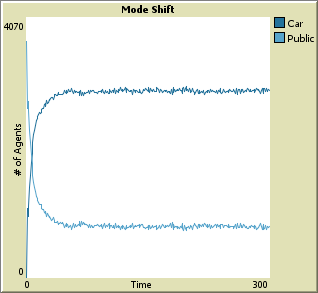
\includegraphics[width=5cm]{Simulation 1 mode shift}
  \caption{Distribution of Agents}
  \end{figure}
 
  \column{2in}
   \begin{figure}

	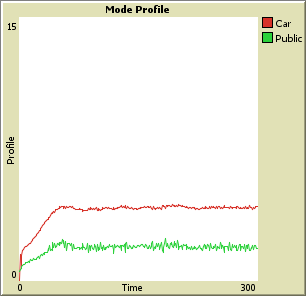
\includegraphics[width=5cm]{Simulation 1 mode profile}

\caption{Mode Profiles}
\end{figure}

 \end{columns}
\end{frame}

\begin{frame}
\frametitle{Results (From Data)}
\begin{columns}[c]
  \column{2in}  % slides are 3in high by 5in wide
  \begin{figure}
  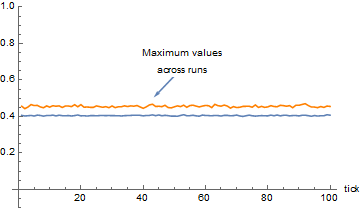
\includegraphics[width=5cm]{average cars avgmin}
  
  \caption{Proportion of Car strategists}
  \end{figure}
 
  \column{2in}
   \begin{figure}

	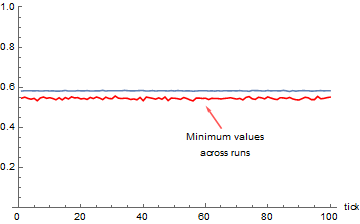
\includegraphics[width=5cm]{average prop avgmin}

\caption{Proportion of public transport strategists}
\end{figure}

 \end{columns}
\end{frame}

\section{Conclusion}
\begin{frame}


\frametitle{Conclusion}

Finally, the goal of this study was to build a model of travel mode choice that is capable of embedding evolutionary game theory to understand the behavior of travelers and the various characteristics included.
Game theory seems to be useful in modeling the relationship between travel modes and Nash equilibrium. Therefore, We are writing a scientific paper based on this work.
\end{frame}
\subsection{Future Work}
\begin{frame}
\frametitle{Future Work}
We can use concepts from machine learning models and artificial intelligence studies, as well as neural networks and genetic algorithms to represent the decision making process of travelers.
\end{frame}
\end{document}
